Caffe is a deep learning framework for research in deep neural
networks. It is widely used across the DNN community
and has become one main platform for neural network algorithm development. 
Two main reasons justify this. Firstly, Caffe supports
many network architectures and different training algorithms for
neural networks. Secondly, Caffe is optimized with GPU acceleration.
This section describes the main operational aspects of Caffe
regarding its parallelization. 
%It is not a functional description of the framework and its capabilities for the design of neural networks. 
The main focus of this section is to describe the neural network 
training algorithm in terms of how the computations happen across 
the network, how the data flow across these layers 
and the different types and levels of parallelism that exist within each layer.

\begin{figure}[]
\centering
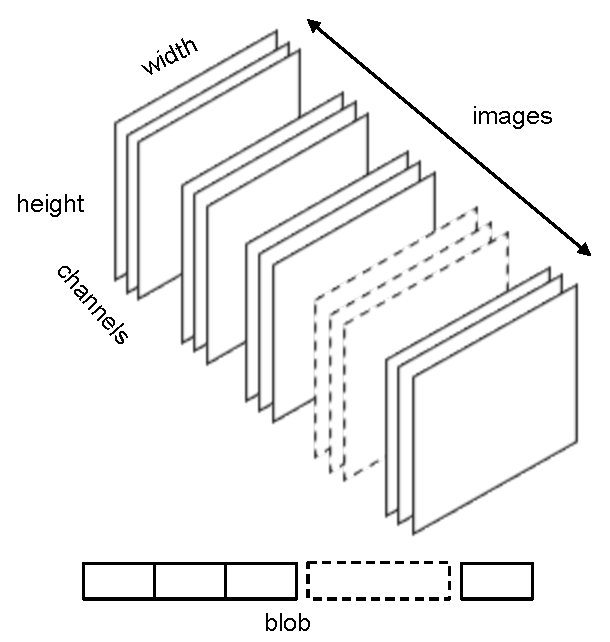
\includegraphics[width=5cm]{figures/blob1.pdf}
\caption{Example of blob structure and data segments within the blob. Each image is composed of data of three channels. Each channel is stored in one blob segment, so that every image occupies three blob segments. Images are stored sequentially one after the other within the blob.}
\label{fig-blob}
\end{figure}
\begin{figure}[]
\centering
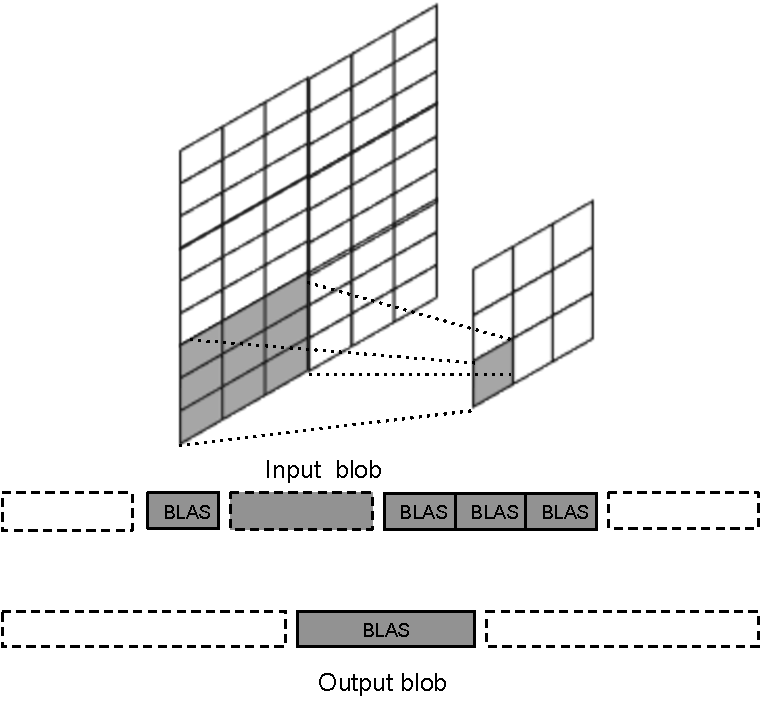
\includegraphics[width=6cm]{figures/blob2.pdf}
\caption{Example of layer transformation and its corresponding blob organization. Every 9 input segments generate the content of one segment in the output blob. This scheme is usual in deep neural networks for dimensionality reduction purposes. Pooling layers (e.g.: Caffe AVERAGE or MAX pooling layers) perform such type of computations.}
\label{fig-blob-trans}
\end{figure}

\subsection{Neural Networks in Caffe}
Caffe allows an user to specify the network structure in a prototext format \cite{protocol-buffer} 
that can capture any kind of arbitrary DAG (directed acyclic graph).
Caffe framework allows users to define their own \emph{Layers} and each layer has a pre-defined generic interface. 
Hence as users compose a network of these Layers it becomes very easily to define extremely complicated graphs in a very compact notation. 
Caffe also allows users to specify all the solver parameters as part of a \emph{Solver} file that is used for the optimization process. 
The optimization process uses back propagation and implements several algorithms such as SGD, ADAGRAD, NESTEROV. 

A network (Net) in Caffe comprises of a set of layers. In a feed-forward network each layer is stacked
such that the output of one layer becomes the input to the next immediate layer in the network graph. 
The first layer processes the input (Data) that is fed to the neural
network. Each of the subsequent layers apply a data transformation 
according to each specific layers computation. The output of Caffe is the 
set of the coefficients in each layer after the network training process is
completed. Regarding the parallelization of the training process, the
main aspects to consider are how the input/output data flow across
the network, the structure of the computation in each layer and the
training algorithm itself.

\subsubsection{Input-Output Data}
Caffe stores and communicates data using blobs. \emph{Blobs} provide a unified memory interface 
holding data; e.g., batches of images, model parameters, and derivatives for optimization.
%The data structure that implements the communication between network layers is the \emph{Blob}. 
Mathematically a Blob is an N-dimensional array stored in a C-contiguous fashion. 
Blobs also conceal the computational and overhead of mixed CPU/GPU operation by synchronizing 
from the CPU host to the GPU device as needed. 
The conventional blob dimensions for batches of image data are number N x channel K x height H x width W. 
For example, if a network is trained on image data, the input data would be organized as a 4-dimensional blob and 
the value at index (n, k, h, w) is physically located at index ((n * K + k) * H + h) * W + w within the sequential Blob data structure.
The first dimension corresponds to the image index in a batch of images and the other
three indicates the number of channels (e.g. 3 for an RGB encoded image) and the image dimensions (height and width). Figure \ref{fig-blob}
shows an example of an input blob. For this case, the blob 
stores one image with 3 data segments, one per each image channel. 
Images are sequentially stored in the blob following this pattern. 
%In respect to computation and parallelization, the blob is a sequential data structure in the form of an array of elements
%that are accessed through a base address plus an offset, given the value of several index dimensions.


\subsubsection{Layer Computation}
Each layer performs a data transformation by operating on the input blobs and generates
output blobs. 
%that is usually based on basic linear algebra operations. 
These operations are computed in a piecewise manner 
throughout the input blob. The input blob/s are organized in
data segments where the linear algebra operations are applied. The
size of the segments is constant and layer dependent. The output
of the computation are blob/s, again organized in fixed size
segments. The computation of a layer is built upon an iterative
structure that traverses the segments in the input blob/s and applies
a specific transformation based on one or more BLAS computations 
on each segment. The output of the processing of one input data 
segment is stored in one segment in the output blob. 
Figure. \ref{fig-blob-trans} shows an example for this computational 
scheme as well as the relation between the input and output blobs 
for a layer computation. Shadowed patches correspond data segments 
in the blobs. In this case, 9 data segments in the input blob are 
used to compute a one segment in the output blob. 

In general, such transformations are implemented using basic algebra 
operations like matrix-$\times$-vector or matrix-$\times$-matrix products and are often referred to as Level 2/3 BLAS operations \cite{BLAS}. 
A layer can be understood as a procedure based on several functions in the 
form of f$_i$(x, W$_i$, b$_i$) = W$_i$x + b$_i$. The layer coefficients 
would correspond to the matrices W$_i$ and vectors b$_i$. Input x would 
correspond to a data segment in the input blob. The training process 
of a neural network optimizes the W$_i$ and b$_i$ coefficients so that 
the network accuracy is maximized for a particular data model.

\subsubsection{Neural Network Training}
The training process of a neural network is based on the gradient
descent algorithm. The algorithm continuously seeks the minimization of a cost function along training epochs, where one epoch 
constitutes of processing all the training data samples. These are 
grouped in batches of fixed size and during every epoch each batch 
is processed in two steps. First, the batch samples are used to 
compute the average error of the network. The samples 
traverse the network where each layer applies its transformation and 
temporally stores its output in a blob. This phase is identified as 
the \emph{forward pass} of the network. Second, the network computes the 
gradient of its transformation as a whole. In this phase, every layer 
applies the chain rule for propagating the derivatives across the layers in the backward direction. From the 
last layer up to the first one in the network, each layer propagates 
its output multiplied by its derivative value. This phase is identified 
as the \emph{backward pass}. Both the forward and backward pass are 
inherently sequential as both the output and the gradients have to 
be propagated through the layers in an upward and downward manner across 
the network. Algorithms \ref{alg-train}, \ref{alg-forw} and \ref{alg-back} 
show the high level structure of the training algorithm as well as 
how the data flow across the layers in the forward and backward pass.
 
%\IncMargin{1em}
\begin{algorithm}
\caption{Iteration of the DNN training algorithm.}
\label{alg-train}
%\SetKwData{Left}{left}\SetKwData{This}{this}\SetKwData{Up}{up}
%\SetKwFunction{Union}{Union}\SetKwFunction{FindCompress}{FindCompress}
\SetKwInOut{Input}{input}\SetKwInOut{Output}{output}
%\KwData{batches}
%\KwResult{batches}
\Input{B, batches}
\Output{Network layer coefficients}
\BlankLine
%\Begin{
%\While{loss not acceptable}{
\For{$b\leftarrow 1$ \KwTo $B$}{
%  \For{$s\leftarrow 1$ \KwTo $S$}{
\BlankLine
    top[1]=layers(1)$\rightarrow$ forward(batches[b]);
\BlankLine
    \For{$l\leftarrow 2$ \KwTo $L$}{
      top[l]=layers(l)$\rightarrow$ forward(top[l-1]);
    }
\BlankLine
    diffs[1]=layers(L)$\rightarrow$ backward(top[L]);
\BlankLine
    \For{$l\leftarrow L-1$ \KwTo $1$}{
      diffs[l]=layers(l)$\rightarrow$ backward(top[l],diffs[l+1]);
    }
updateCoefficients(layers, top, diffs);
  }
%}
%loss = evaluateNetwork(layers);
%}
%}
\end{algorithm}
%\DecMargin{1em}

Algorithm \ref{alg-train} corresponds to one training iteration. 
Each data batch \emph{b} is propagated through the network. 
First layer processes the batch and outputs the first transformation 
for each sample in it. This is than forwarded to the 
second layer to apply the next transformation. This process continues 
until all layers have applied their transformation. The last layer 
of the network is the one responsible to check the output of the 
network and evaluate the network accuracy. The loop in line 3 implements 
the batch network computation, the network forward phase.
This loop is inherently sequential and each layer 
transformation happens within the \emph{forward} call. The output of 
this call is stored in vector \emph{top} for all data samples in the 
batch. Each \emph{forward} invocation uses as input the \emph{top} 
produced by the previous layer. Loop in line 6 corresponds to the 
computation of network gradients. Once the network has been evaluated 
with one batch, the algorithm computes every layers gradient 
with respect its input. This process seeks the minimization 
of the network error. This loop is also inherently sequential and 
the \emph{backward} call computes the layer gradient, \emph{diffs}. 
This process requires both the evaluation of the layer transformation 
(\emph{top}) and the previous gradient computed in the immediate previous 
layer (\emph{diffs}) in backward manner. It corresponds to the network 
backward phase. Once both the forward and backward phases are completed, 
the training algorithm updates the network coefficients in all layers. 
This corresponds to line 8 and procedure call to \emph{updateCoefficients}.

\begin{algorithm}
\caption{Layer forward phase}
\label{alg-forw}
%\SetKwData{Left}{left}\SetKwData{This}{this}\SetKwData{Up}{up}
%\SetKwFunction{Union}{Union}\SetKwFunction{FindCompress}{FindCompress}
\SetKwInOut{Input}{input}\SetKwInOut{Output}{output}
\Input{Bottom blob (S, N+1, $D_1, D_2$, $\dots$, $D_N$)}
\Output{Top blob for the layer transformation}
\BlankLine
\For{$s \leftarrow 1$ \KwTo $S$}{
\BlankLine
\For{$d_1 \leftarrow 1$ \KwTo $D_1$}{
  \For{$d_2 \leftarrow 1$ \KwTo $D_2$}{
    \dots 
\BlankLine
    \For{$d_N \leftarrow 1$ \KwTo $D_N$}{
      top[f(s, $d_1,d_2$, $\dots$, $d_N$)]=\textbf{BLAS}(W($d_1,d_2$, $\dots$, $d_N$), b($d_1,d_2$, $\dots$, $d_N$), bottom[g(s, $d_1,d_2$, $\dots$, $d_N$)]);
}
}
}
}
\end{algorithm}

\begin{algorithm}
\caption{Layer backward phase}
\label{alg-back}
%\SetKwData{Left}{left}\SetKwData{This}{this}\SetKwData{Up}{up}
%\SetKwFunction{Union}{Union}\SetKwFunction{FindCompress}{FindCompress}
\SetKwInOut{Input}{input}\SetKwInOut{Output}{output}
\Input{Gradient w.r.t. top blob (S, N+1, $D_1, D_2$, $\dots$, $D_N$)}
\Output{Gradient w.r.t. to bottom blob}
\BlankLine
\For{$s \leftarrow 1$ \KwTo $S$}{
\BlankLine
\For{$d_1 \leftarrow 1$ \KwTo $D_1$}{
  \For{$d_2 \leftarrow 1$ \KwTo $D_2$}{
\BlankLine
    \dots 
\BlankLine
    \For{$d_N \leftarrow 1$ \KwTo $D_N$}{
      diffs\_bottom[f(s, $d_1,d_2$, $\dots$, $d_N$)]=\textbf{BLAS}(W($d_1,d_2$, $\dots$, $d_N$), b($d_1,d_2$, $\dots$, $d_N$), top[h(s, $d_1,d_2$, $\dots$, $d_N$)], diffs\_top[g(s, $d_1,d_2$, $\dots$, $d_N$)]);
}
}
}
}
\end{algorithm}

Algorithm \ref{alg-forw} corresponds to the description of the structure 
of one layer transformation. In general, the layer computation is organized 
in a nest of loops that traverse the \emph{N+1} dimensions (\emph{S, D$_1$, 
D$_2$, \dots, D$_N$}) of the layer input blob \emph{bottom} and produces 
a transformation stored in the output blob \emph{top}. The first dimension 
corresponds to the data samples in the batch. These are indexed with the 
variable \emph{s}.  According to layer specific functions 
(\emph{f} and \emph{g} in line 5 of the algorithm), 
data segments in the input/ouput blobs are processed through basic linear 
algebra transformations (\emph{BLAS} call in line 5) that are also 
dependent to the data segment being processed (\emph{W} and \emph{b} 
depend on the loop induction variables). Algorithm 
\ref{alg-back} follows a very similar structure, but operating with 
blobs that store the gradient computation (\emph{diffs\_bottom} and 
\emph{diffs\_top}).


\begin{figure*}[]
\centering
%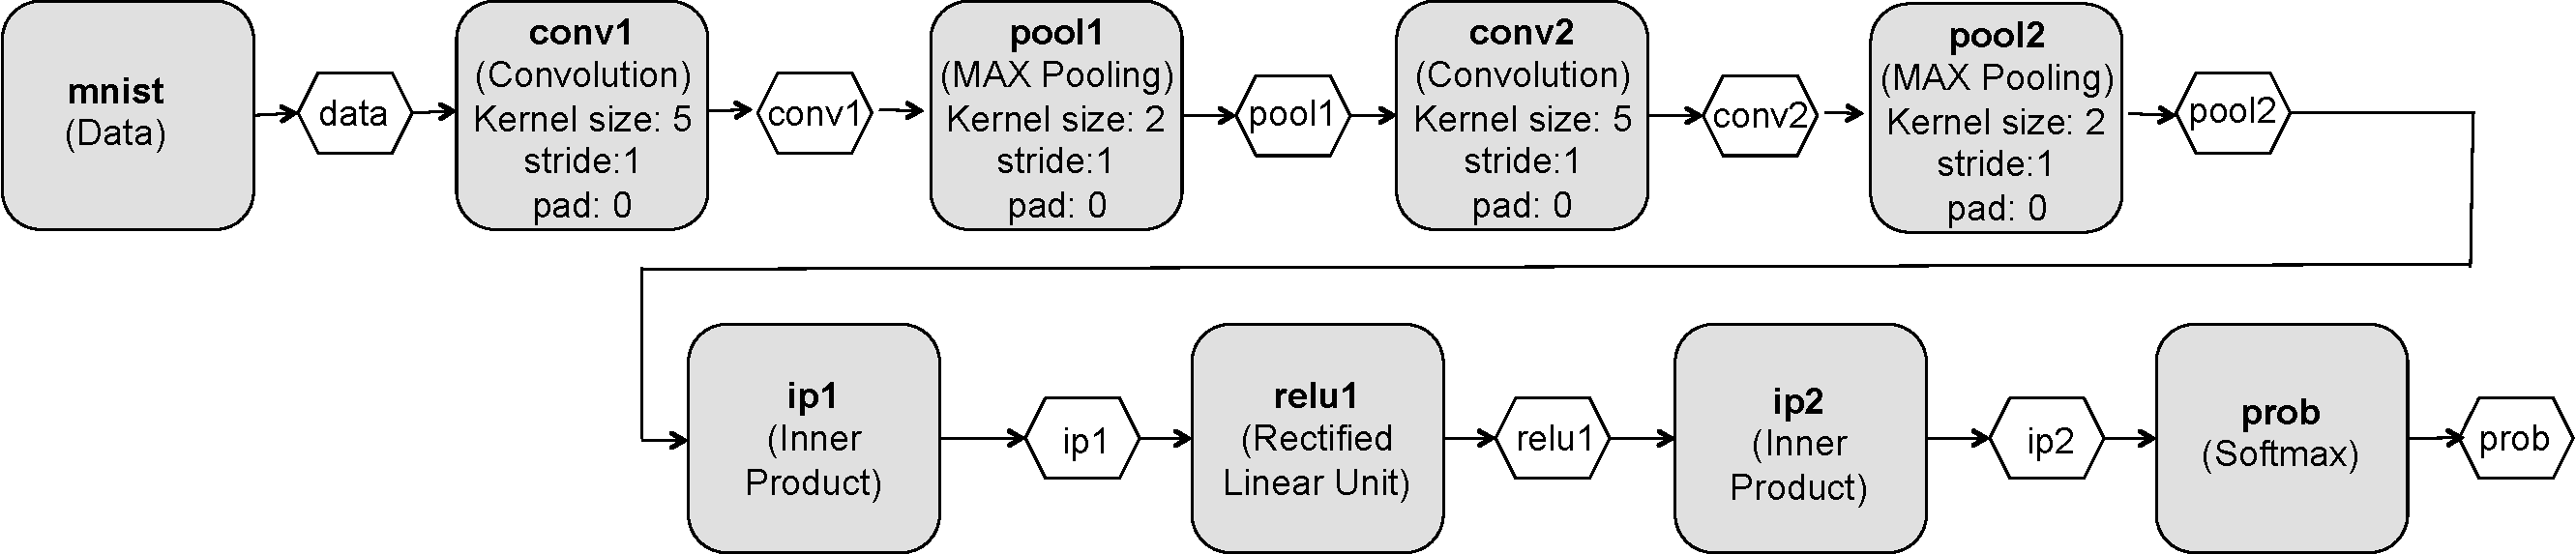
\includegraphics[width=\textwidth]{figures/mnist.pdf}
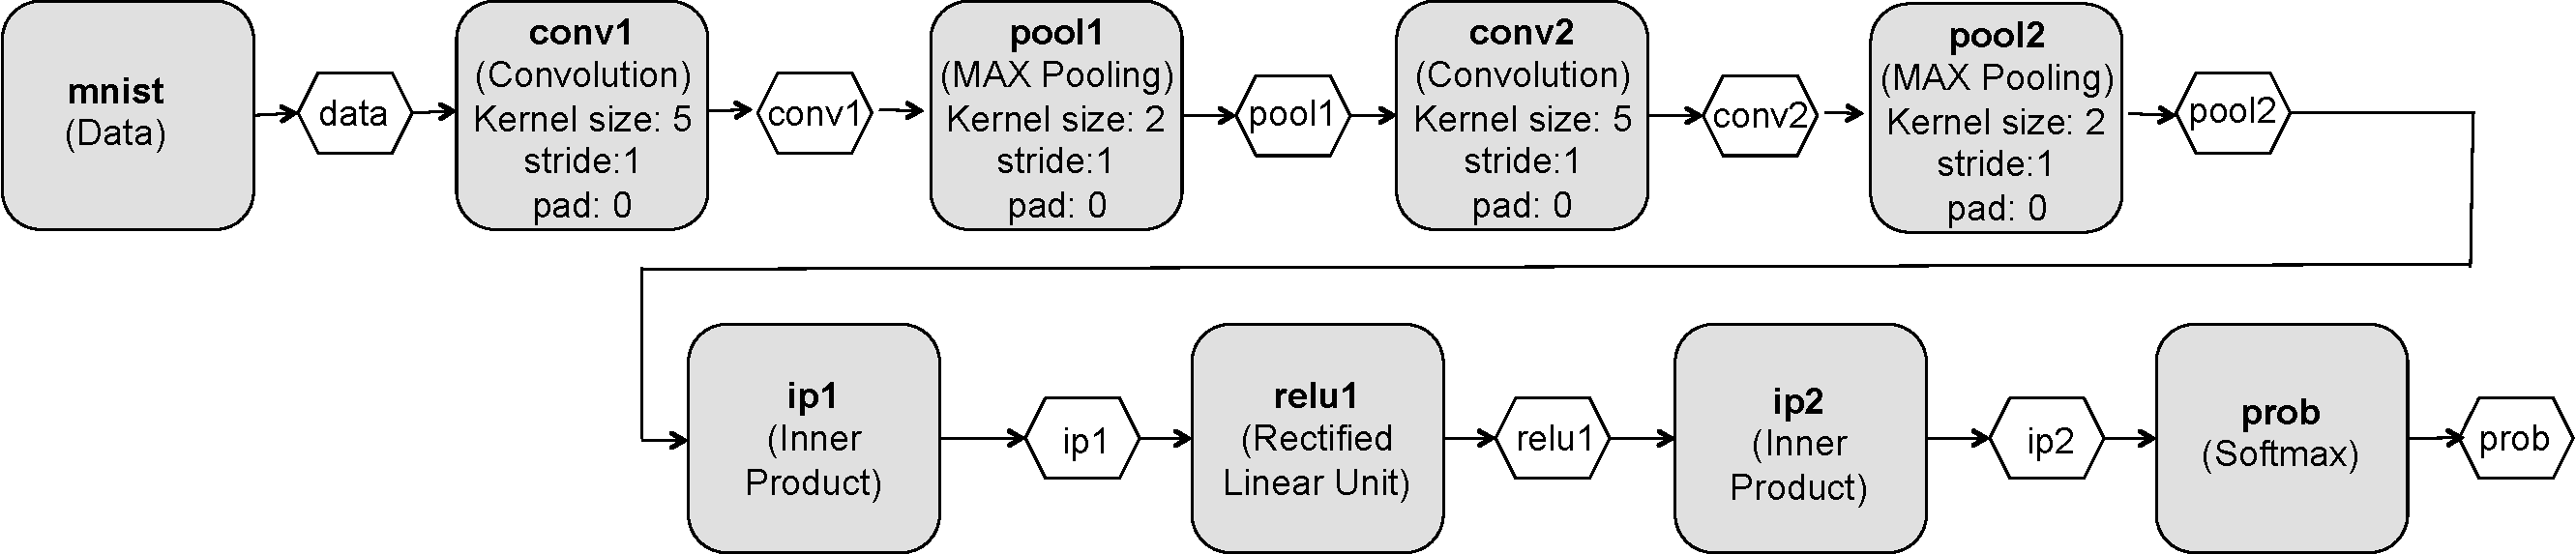
\includegraphics[width=13.5cm]{figures/mnist.pdf}
\caption{MNIST network.}
\label{fig-mnist}
\end{figure*}

\begin{figure*}[]
\centering
%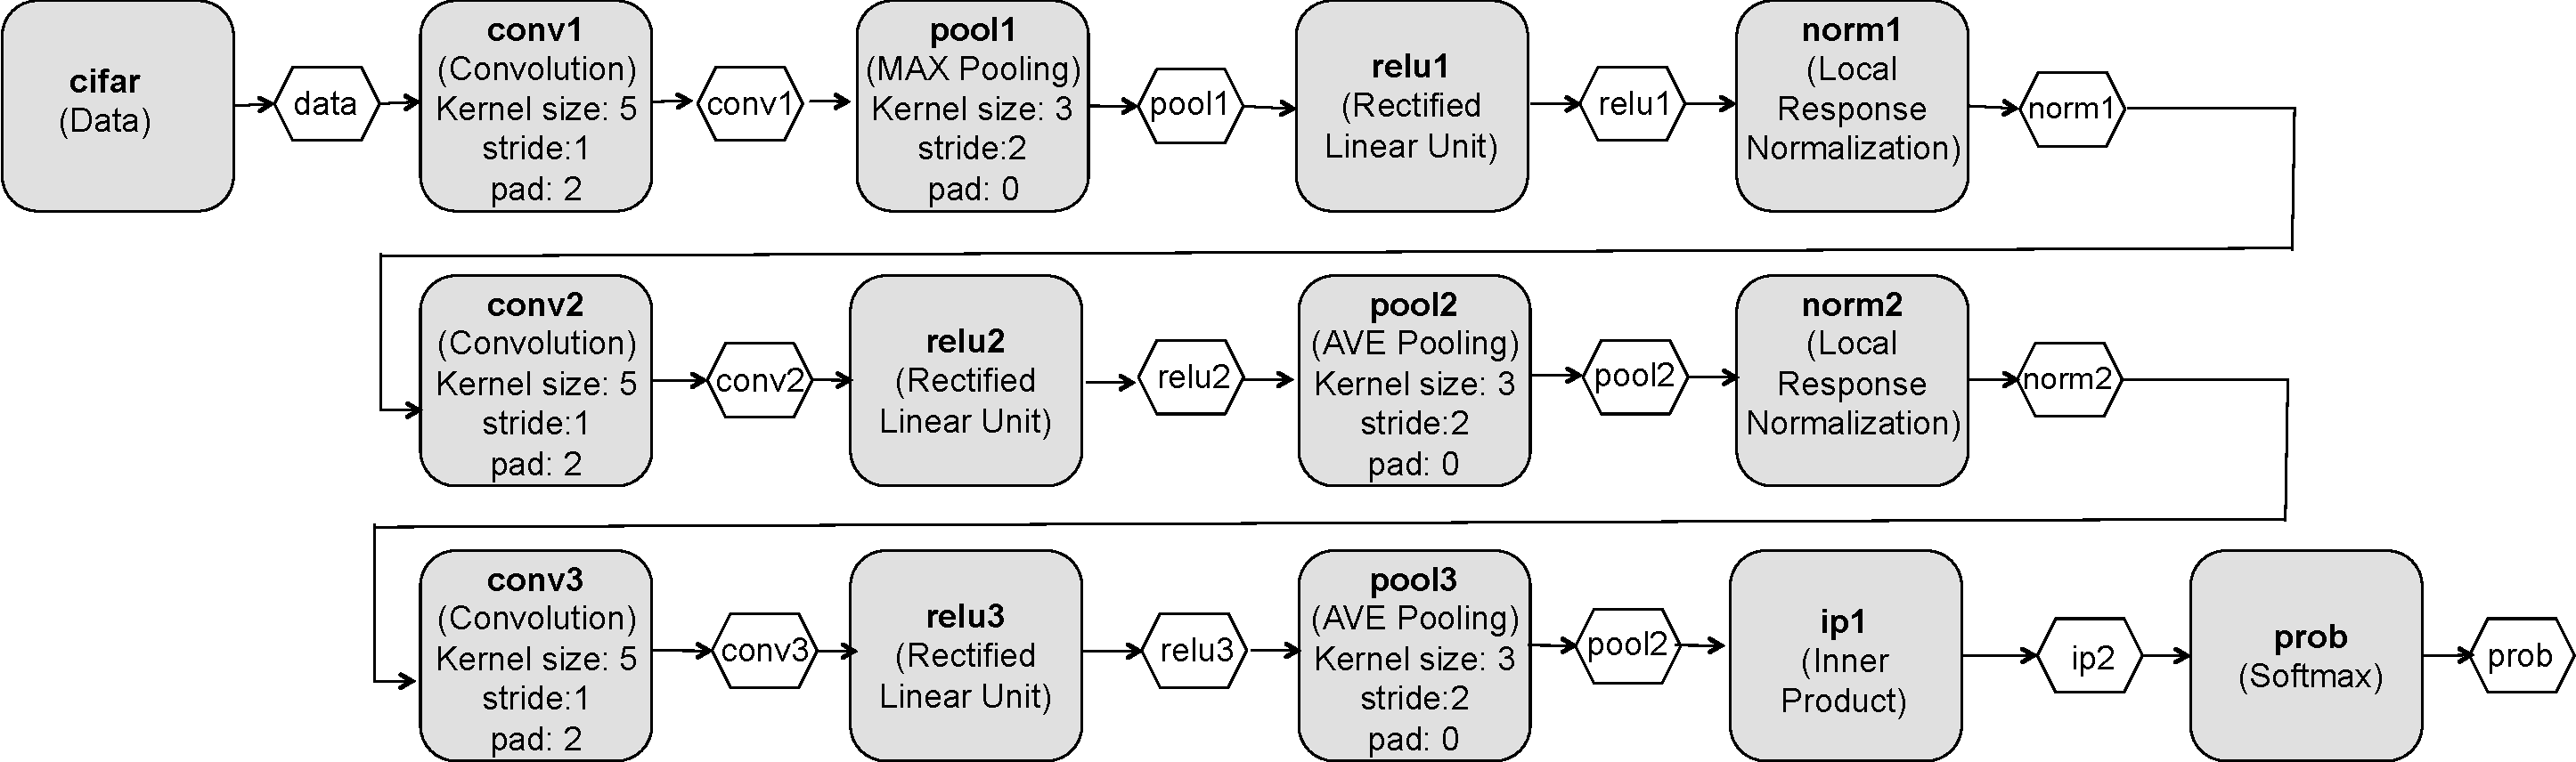
\includegraphics[width=\textwidth]{figures/cifar.pdf}
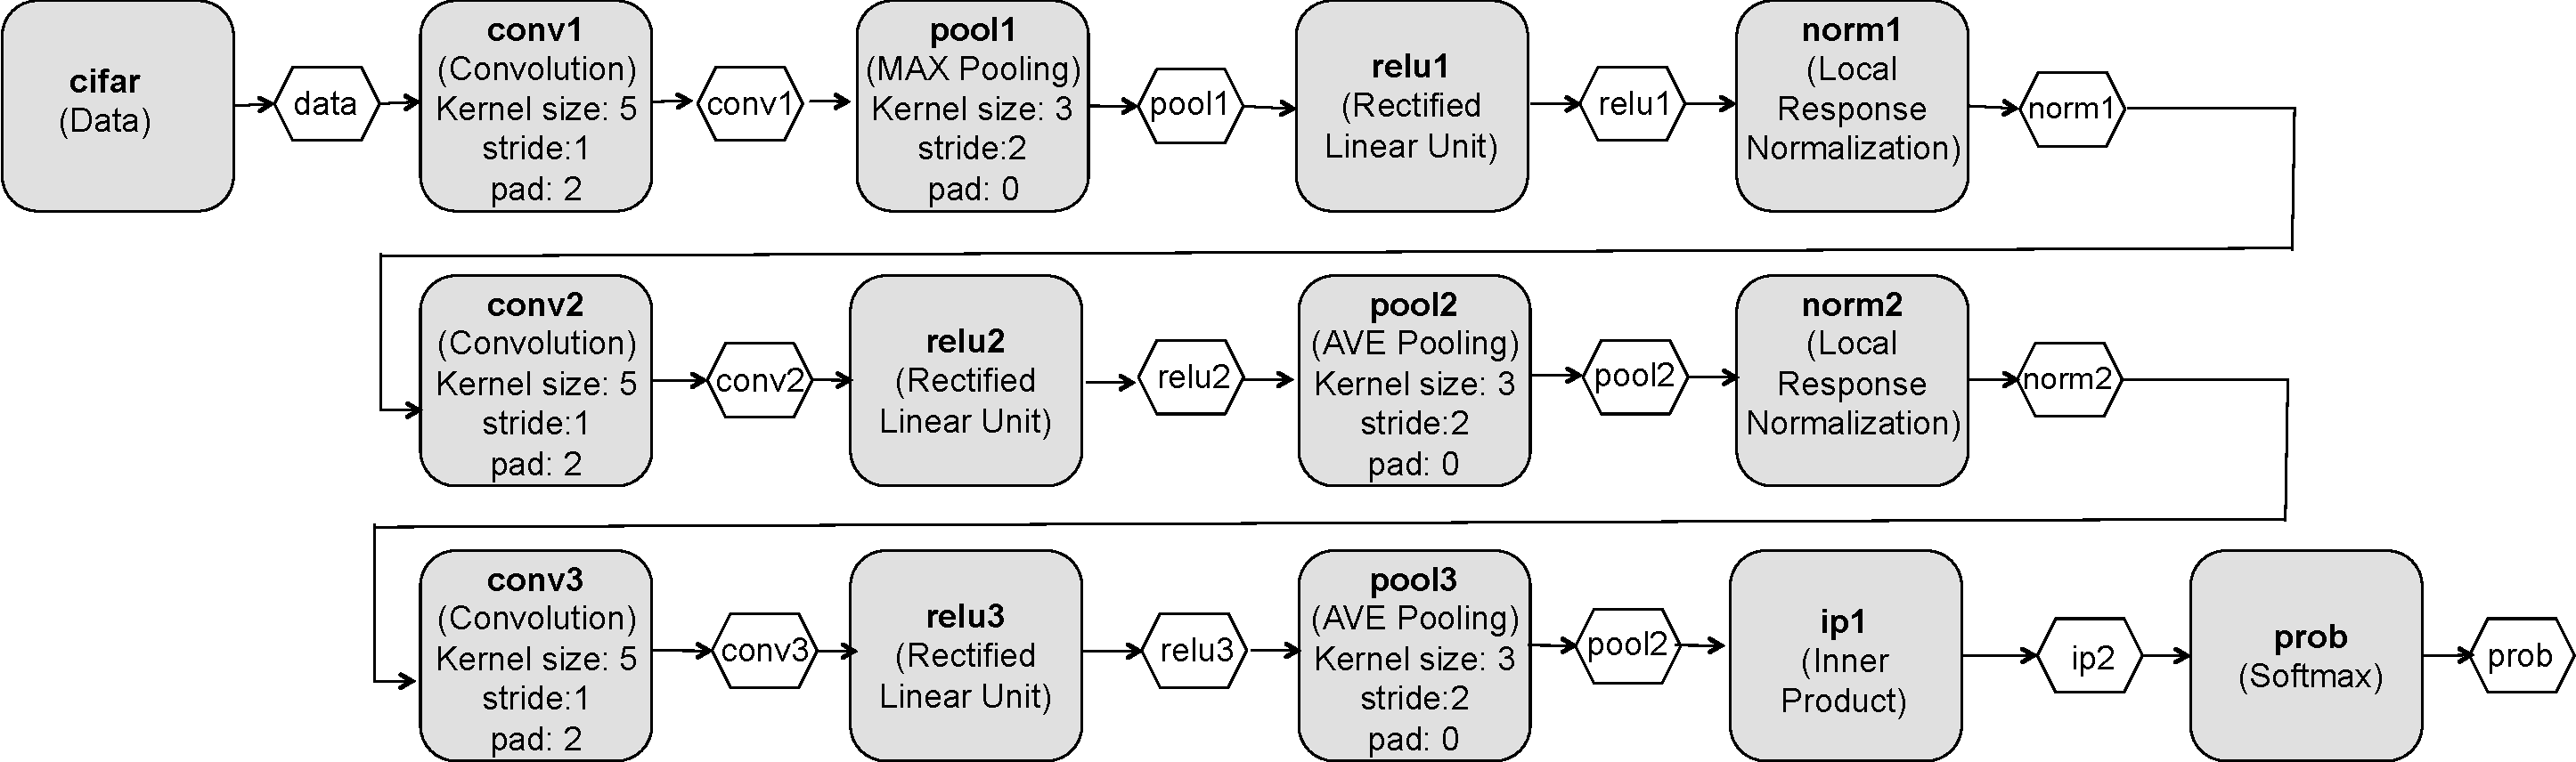
\includegraphics[width=15cm]{figures/cifar.pdf}
\caption{CIFAR-10 network.}
\label{fig-cifar}
\end{figure*}

\subsection{Network Examples: MNIST and CIFAR-10}
The MNIST \cite{Deng2012, MNIST} and CIFAR-10 \cite{CIFAR10} datasets are standard datasets for 
computer vision. The MNIST dataset is composed of 60,000 images, each of dimension 28$\times$28 pixels 
of handwritten digits for training and 10,000 test examples. 
The Caffe distribution includes the LeNet \cite{LeNet} network for generating an image 
classifier for this dataset. Given an a handwritten digit, 
the network outputs which digit is represented (e.g.: 0 \dots 9). 
The CIFAR-10 is a CNN (Convolution Neural network) \cite{CNN} included in the Caffe distribution
that performs as an image classifier for the CIFAR dataset. CIFAR is 
composed of 60,000 32$\times$32 color images with 10 classes: 
\emph{airplane, automobile, bird, cat, deer, dog, frog, horse, ship, 
truck} with 6000 images per class. Both the networks are built with  
a subset of the available layers within Caffe. 

\subsubsection{Types of Layers}
Caffe supports a great variety of network layers. The following 
paragraph describes the layers that are mostly used for computer vision, and 
in particular, for the two example networks studied in this paper.

The \textbf{Data Layer} corresponds to the first layer in the 
network. This layer is responsible of fetching the data in batches and 
feeding it to the network. The \textbf{Convolutional Layer} applies 
a group of convolutions to an image. Its parameters are the size of the 
convolutional patch and the stride to apply along the image, among others. 
In general, the coefficients in this type of layer are learnt so that 
they capture what are the relevant data features 
for the image classification. The \textbf{Pooling Layer} usually 
follows the convolutional layer. In general, this layer applies an averaging 
function over a subset of data points. The most usual functions are the 
MAX pooling function, when the pooling layer selects the maximum value for the 
subset, and the AVERAGE function, when the pooling layer computes the average 
value of the subset. The \textbf{Local Response Normalization Layer} 
performs a local normalization over a local region in the image. 
This normalization can happen across the image channels or within the image 
channels. The \textbf{Rectified Linear Unit Layer (ReLU)} computes 
the max(x,0) function for each element in its input blob. 
The \textbf{Inner Product Layer} also identified as a fully-connected layer, 
performs a vector product between its input and coefficients.  
The \textbf{Loss and Accuracy Layers} correspond 
to the deepest layers in the network. They are responsible for evaluating the 
loss function for the gradient computation and the overall network accuracy.

\subsubsection{Networks}
The aim of this section is to briefly introduce the two networks 
used in this paper. The section describes the network layers and characterizes 
them in terms of feature learning layers and dimensionality reduction 
layers. Regarding the parallelization, it is important to notice that 
the deeper the layers, the smaller the size of the input/output blobs. 
Thus, the level in the network will affect the work granularity of the 
existing parallelism within the layer. 

Figure \ref{fig-mnist} shows the layer composition for the MNIST network. 
This network is composed of an initial data layer followed by the 
combination of two instances of convolutional and pooling layers. The 
convolutional layers are responsible for feature learning while the 
pooling layers correspond to dimensionality reduction. 
This is followed by a inner product layer (ip) and ReLU layer which furthermore reduces the dimensionality 
of the data traversing the network, until the last inner product layer which 
outputs a vector of 10 elements, one per digit class. The last layer corresponds to a loss layer.

Figure \ref{fig-cifar} shows the layer composition for the CIFAR network. 
As in the previous network, the first layer is a data layer, followed by 
the combination of convolutional, ReLU and pooling layers. Again, convolutional 
layers perform the feature learning and pooling layers perform the 
dimensionality reduction. The ReLU layer controls the saturation of 
the output of the convolutional coefficients. CIFAR also includes 
normalization layers between the first two instances of convolution and pooling 
layers.  The inner product layer (ip) and loss layer (SoftMax) are the last layers of the network. 

